%---
\section{Site and Environment}

The \DSks\ detector, \Urania, and \Aria\ sub-project sites have been selected based on the scientific requirements of the sub-projects and the available on-site resources.  Agreements for siting equipment and systems have been established with the primary landowners or hosting institution of each site as documented by the Supplementary Documents included with the proposal. The permitting process for each of the sites has begun, or in some cases concluded, and is expected to proceed as defined in the project schedule.  The \DSks\ detector will be located in Hall C of \LNGS. The overall layout of the facility is shown in Figure~\ref{fig:Overall-Design}.  The \Urania\ facility will be located on land owned by Kinder Morgan that is adjacent to the gas processing facility handling the feed gas stream containing the \UAr.  A preliminary layout of the Urania facility is shown in Figure~\ref{fig:UraniaLayout}.  The \Aria\ project is already under construction at the Monte Sinni mine of the Carbosulcis Company in Sardinia, Italy, where a vertical shaft has been completely refurbished and outfitted to accommodate \AriaSeruciHeight\ tall distillation columns.

\begin{figure} [!t]
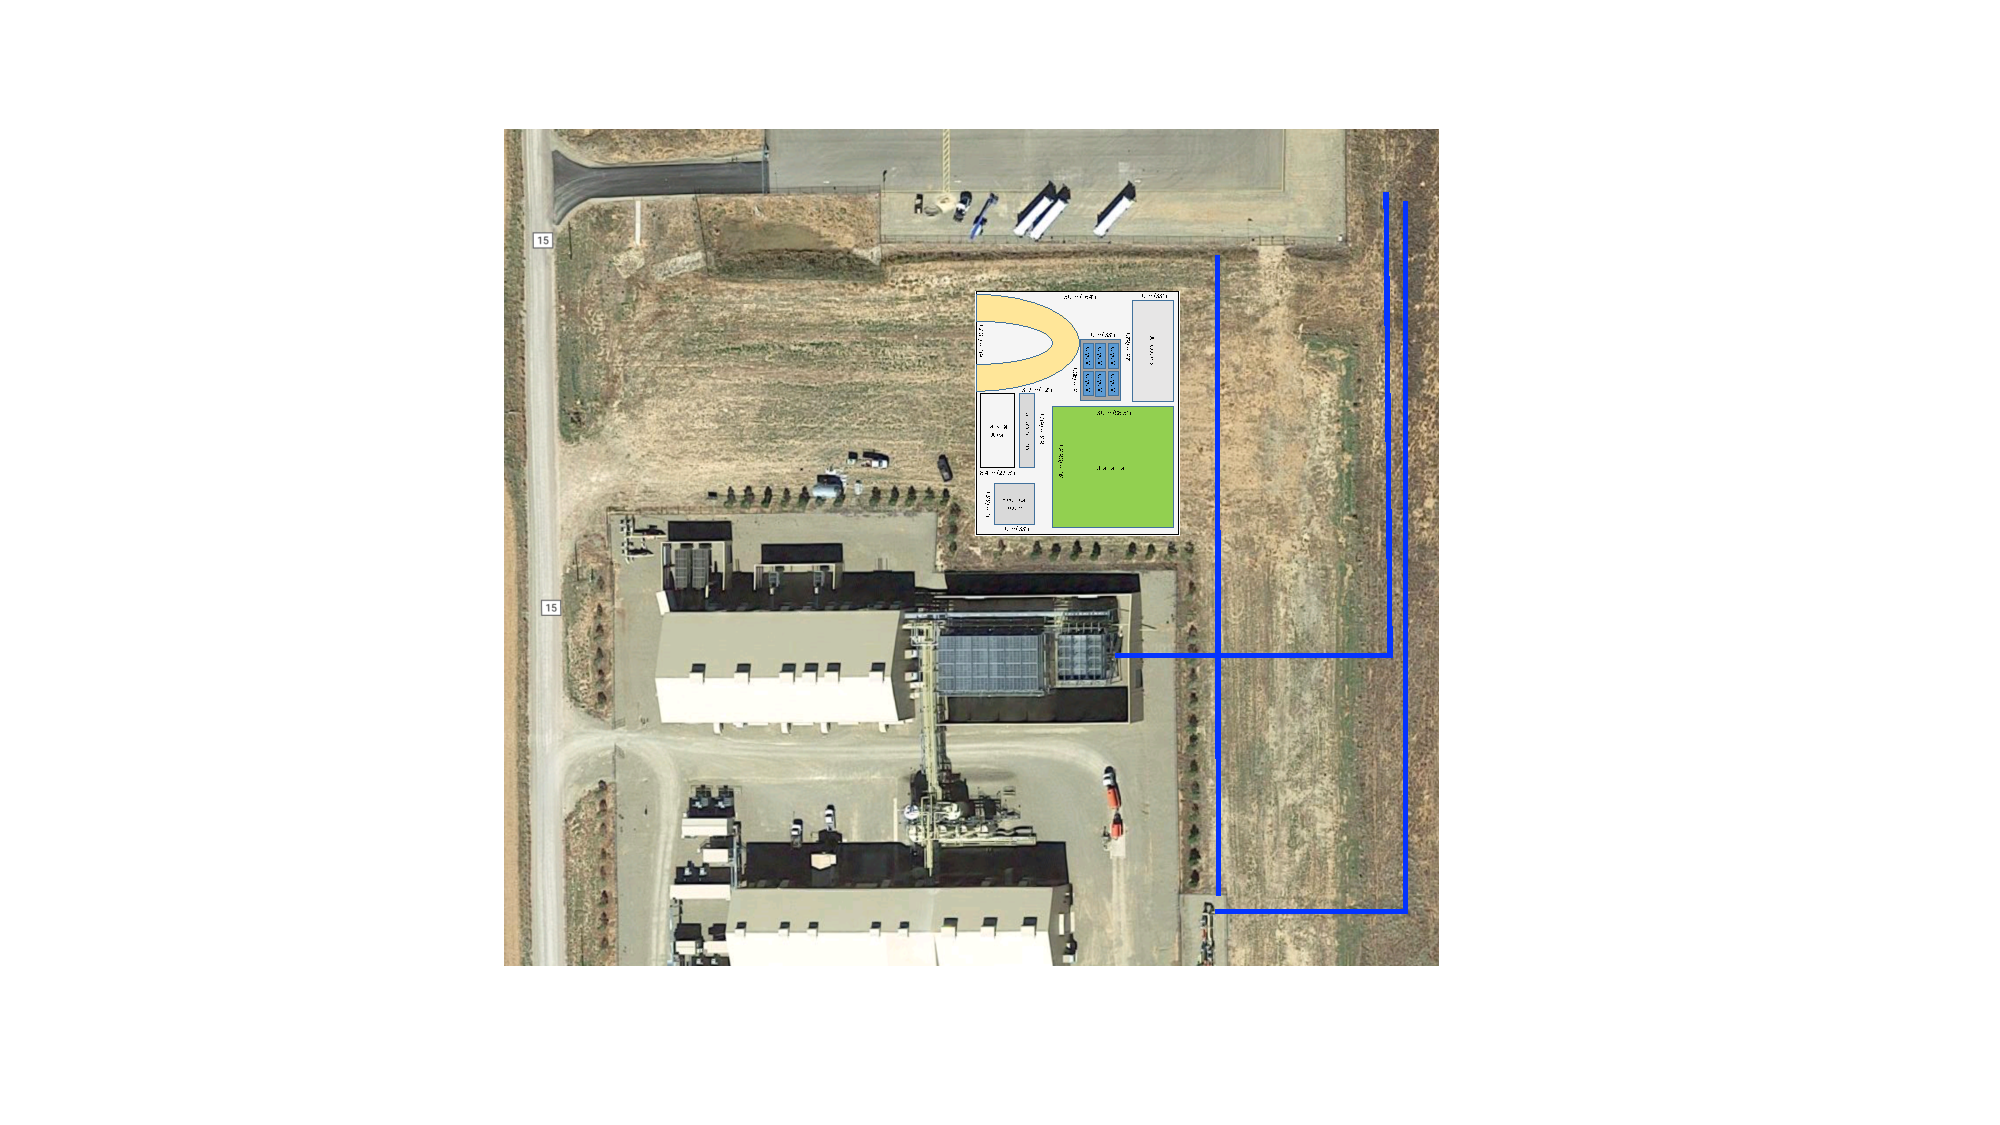
\includegraphics[width=0.99\columnwidth]{./Figures/Urania-FacilityLayout.pdf}
\caption[Preliminary layout of \Urania\ facility]{Preliminary layout of the \Urania\ facility within the approved facility boundary adjacent the Kinder Morgan CO2 Company gas processing facility.}
\label{fig:UraniaLayout} 
\end{figure} 

The \GADMC\ will designate a Work Group charged with ensuring that proper permitting and site assessments are performed in line with the requirements of the host site and following all local and national regulations.